Se implementaron dos efectos, eco simple y reverberación, siguiendo el método descrito por M. Schroeder\footnote{M. Schroeder, ``Natural Sounding Artificial Reverberation'', Journal of the Audio Engineering Society, vol. 10, no. 10, 1962. [Accessed 9 May 2020].}. Para el eco se utilizó una sola linea de delay mostrada en la Figura (\ref{delay}).
\begin{figure}[H]
	\centering
	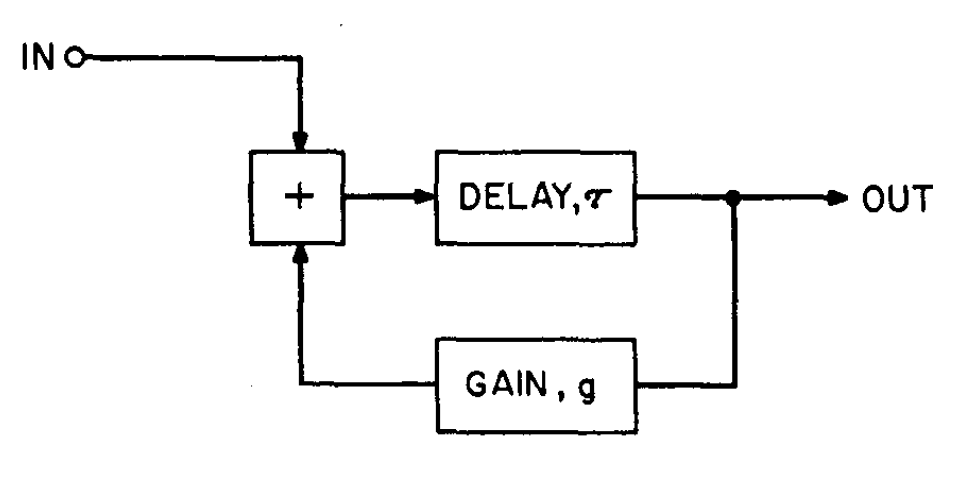
\includegraphics[width=0.7\textwidth]{ImagenesEjercicio6/delay.png}
	\caption{Linea de retardo.}
	\label{delay}
\end{figure}

Los parámetros para configurar este efecto son los de delay time $\tau$, el cual denota el retardo de la línea; y decay factor $g$, el cual describe la ganancia del lazo. Se puede modelizar el tiempo en el cual el sonido decae por $60 \ dB$, $T$, como

\begin{equation}
T = \frac{3*\tau }{-log_{10} | g | }
\label{delayeq}
\end{equation}

Luego, se utilizó el modelo propuesto por M. Schroeder mostrado en la Figura (\ref{rev}) para implementar la reverberación, con cuatro lineas de retardo en paralelo, seguidas de dos filtros pasa todo con linea de retardo, los cuales aumentan la densidad de los ecos sin afectar la ganancia del sistema en función de la frecuencia.

\begin{figure}[H]
	\centering
	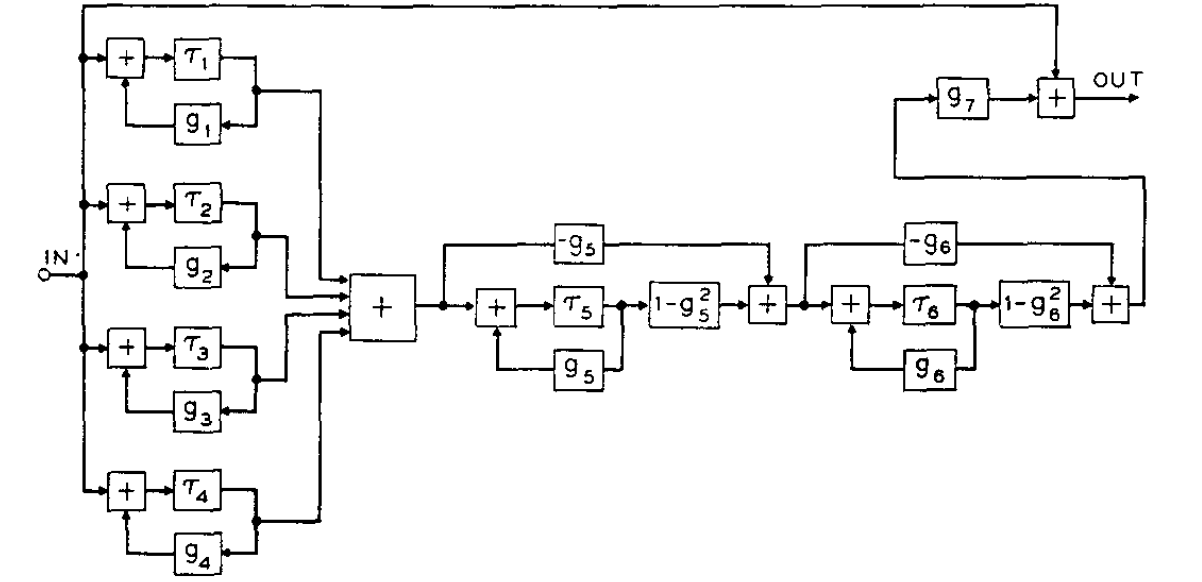
\includegraphics[width=0.7\textwidth]{ImagenesEjercicio6/rev.png}
	\caption{Filtro all-pass con linea de retardo.}
	\label{rev}
\end{figure}

Se utilizaron los parámetros sugeridos por Schroeder detallados a continuación\footnote{John M. Chowning, \href{https://ccrma.stanford.edu/sites/default/files/user/jc/fm_synthesispaper-2.pdf}{The Synthesis of Complex Audio Spectra by Means of Frequency Modulation.} 1973.}

\begin{table}[H]
\centering
\begin{tabular}{@{}cc@{}}
\toprule
Parámetro & Sugerencia \\ \midrule
$\tau_5$ & $5 \ ms$ \\
$\tau_6$ & $1.7 \ ms$ \\
$g_5$ & $0.7$ \\
$g_6$ & $0.7$ \\
$\tau_1$ & $101.560 \ ms$ \\
$\tau_2$ & $113.356 \ ms$ \\
$\tau_3$ & $122.426 \ ms$ \\
$\tau_4$ & $131.54 \ ms$ \\ \bottomrule
\end{tabular}
\caption{Parámetros utilizados según las referencias empleadas.}
\end{table}

Luego, se ajustaron los valores de $g_1$ hasta $g_4$ según (\ref{delayeq}). Finalmente, para el eco se le pide al usuario que ingrese el delay time y el decay factor, denominados en el programa con las letras $T$ y $D$. Para la reverberación, se le pide al usuario el tiempo de reverberación, el cual es el tiempo en el que el sonido decae $60 \ dB$, denotado con la letra $T$; y el mix factor, detallado en la Figura (\ref{rev}) como $g_7$, denotado en el programa con la letra $M$.